\tikzsetnextfilename{orthodromic_distance}
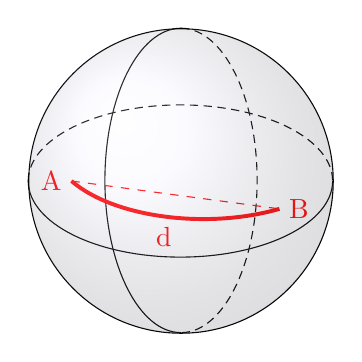
\begin{tikzpicture}


\tikzset{
	spherical/.pic={
      \draw (-0.0352778*#1,0) arc (180:360:#1 pt and 0.5*#1 pt);
      \draw[densely dashed] (-0.0352778*#1,0) arc (180:0:#1 pt and 0.5*#1 pt);
      \draw (0,0.0352778*#1) arc (90:270:0.5*#1 pt and #1 pt);
      \draw[densely dashed] (0,0.0352778*#1) arc (90:-90:0.5*#1 pt and #1 pt);
      \coordinate (A) at (-0.0252778*#1,0);
      \draw[red, line width=0.5mm]  (A) arc (210:300:#1 pt and 0.5*#1 pt) coordinate (B) node[midway, below]{d};
      \node[red, left] at (A) {A};
      \node[red, right] at (B) {B};
      \draw[red, dashed] (A) -- (B);

      \draw (0,0) circle (#1 pt);
      \shade[ball color=blue!10!white,opacity=0.20] (0,0) circle (#1 pt);
    }
}

\pic [local bounding box=spher]  at (0,0) {spherical=55};

\end{tikzpicture}
